\documentclass[oneside,a4paper,12pt]{extarticle}

%\newcommand{\managementComputerName}{Raspberry Pi 2 Model B}

\usepackage{mathtools}
\usepackage{Format}
\usepackage{listings}
\usepackage{wrapfig}
\usepackage[table]{xcolor}

\definecolor{Gray}{gray}{0.85}

\usepackage{titlesec}
\setcounter{secnumdepth}{4}
\titleformat{\paragraph}
	{\normalfont\normalsize\bfseries}{\theparagraph}{1em}{}
\titlespacing*{\paragraph}
	{0pt}{3.25ex plus 1ex minus .2ex}{1.5ex plus .2ex}

\usepackage{listings}
\lstset{
	frame = none, 
	language=, 
	basicstyle=\small,
	aboveskip=0.2cm,
	belowskip=-0.5cm
	%xleftmargin=\parindent,
	}

\usepackage{textcomp}
\usepackage{apacite}
\bibliographystyle{apacite}


\begin{document}
\pagenumbering{Roman}

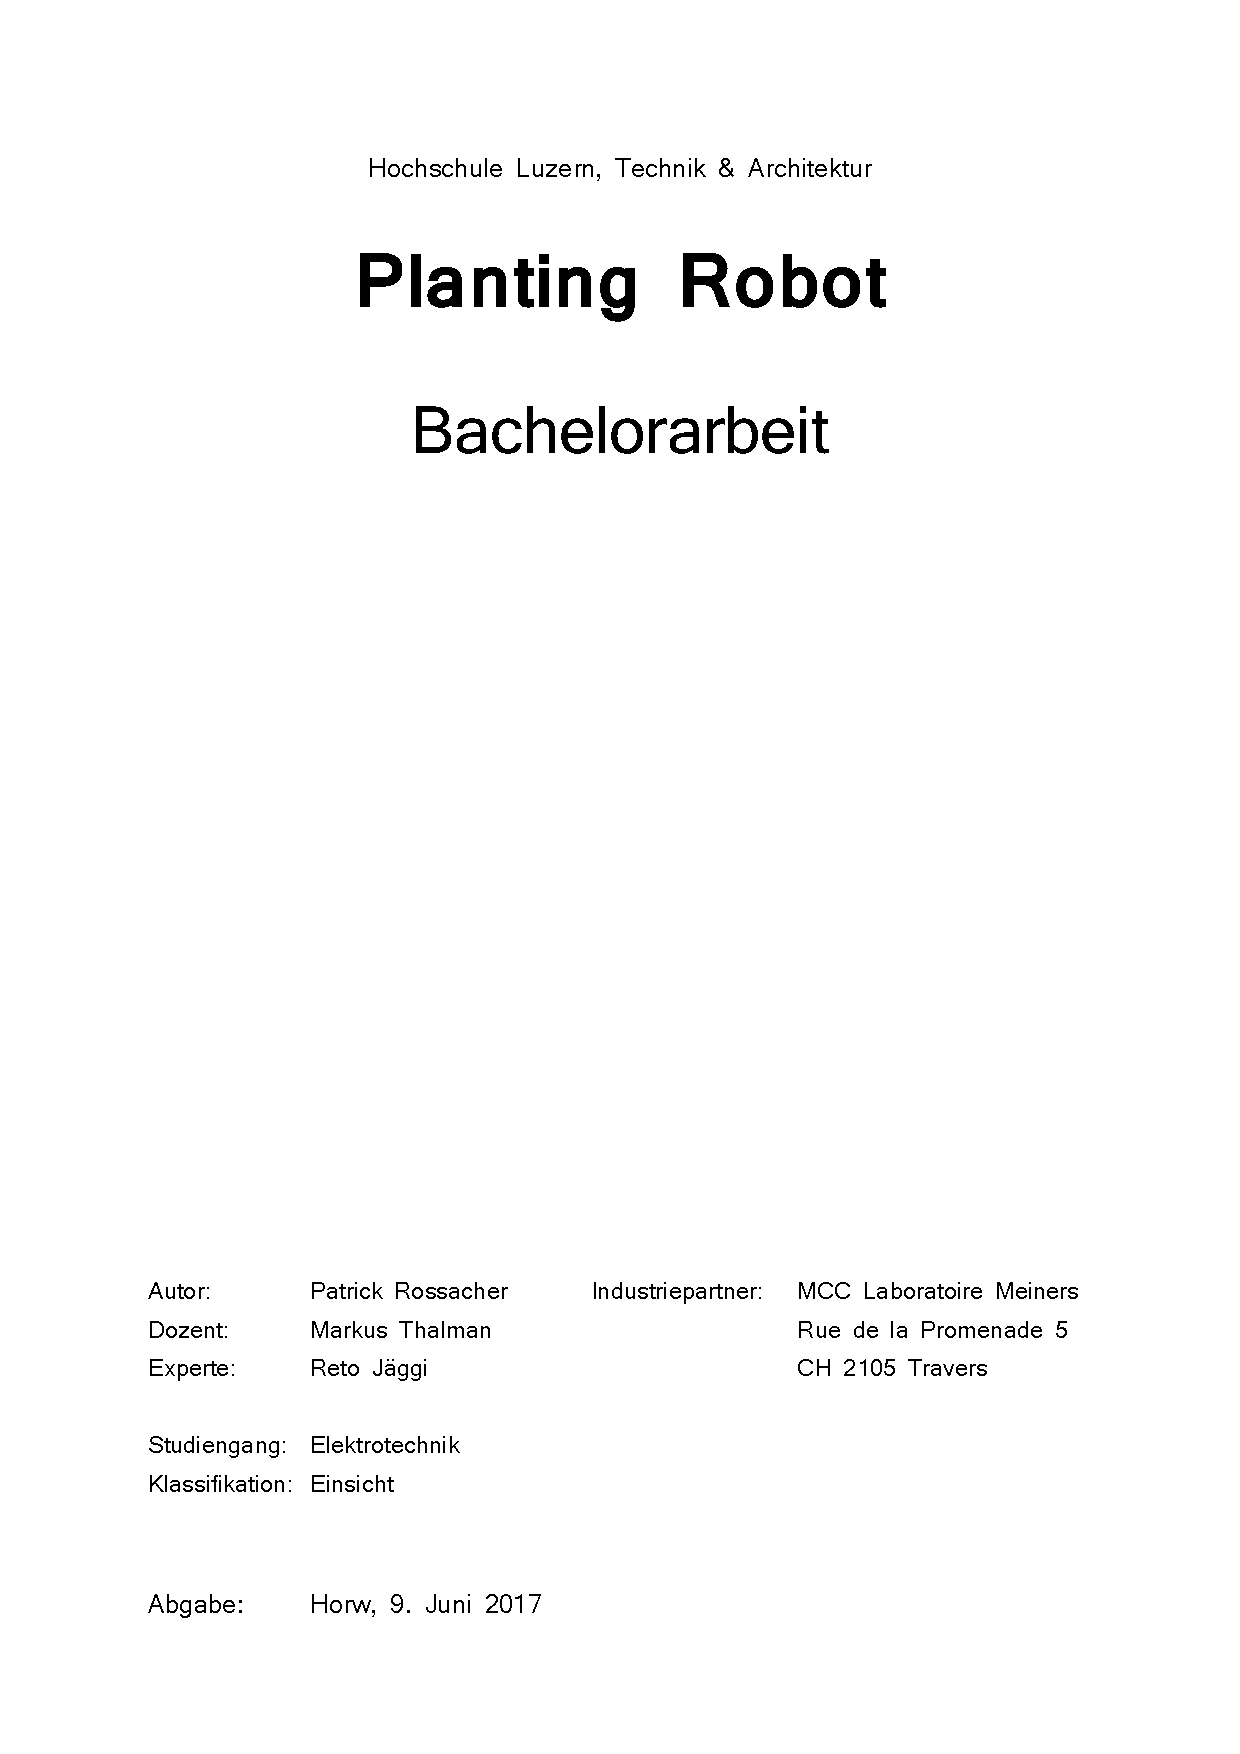
\includepdf{Illustrationen/0-Vorspann/Titelblatt.pdf}
\input{Kapitel/0_Vorspann/0.1_Redlichkeitserklärung}
\newpage
\fontsize{12}{15}
\selectfont
\sloppy
%\begin{sffamily}
\renewcommand{\contentsname}{Inhaltsverzeichnis}
\tableofcontents
%\end{sffamily}
\newpage
\begin{comment}
	\phantomsection\addcontentsline{toc}{section}{Abbildungsverzeichnis}

	\begin{sffamily}
	\listoffigures % Abbildungsverzeichnis
	\end{sffamily}	Inhalt...
\end{comment}

\begin{comment}
	\phantomsection\addcontentsline{toc}{section}{Tabellenverzeichnis} 
	\begin{sffamily}
	\newpage
	\listoftables % Tabellenverzeichnis
	\end{sffamily} 	Inhalt...
\end{comment}

\newpage
%\begin{sffamily}
\phantomsection\addcontentsline{toc}{section}{Glossar} 
\section*{Abkürzungsverzeichnis}\label{dok:glossar}
\begin{table}[H]
	\begin{tabular}{|L{2.5cm}|L{13cm}|}

		\hline	
		\textbf{ABS} & Acrylnitril-Butadien-Styrol. Thermoplast der in der Additiven Fertigung verwendet wird.\\
		
		\hline	
		\textbf{DC} & Direct Current\\

		\hline
		\textbf{FDM} & Fused Deposition Modeling. 3D-Druckverfahren: Kunststoff wird durch eine oder mehrere Düsen extrudiert und zu Bauteillagen zusammengeführt.\\
		
		\hline
		\textbf{GND} & Ground\\
		
		\hline
		\textbf{HSLU T\&A} & Hochschule Luzern für Technik und Architektur\\ 
		
		\hline
		\textbf{KDS} & Kinetis Design Studio\\

		\hline
		\textbf{LED} & Light-emitting diode\\
		
	 	\hline
	 	\textbf{PAIND} &  Industrieprojekt (Modul der HSLU) \\ 
	 	
	 	\hline
	 	\textbf{PCB} &	Printed Circuit Board\\
				
		\hline
		\textbf{RTOS} & Real Time Operating System \\
		
		\hline
		\textbf{SoC} &	System on Chip\\
		
		\hline
		\textbf{SWD} &	Serial Wire Debug\\
		
		\hline
		\textbf{UART} &	Universal Asynchronous Receiver Transmitter\\
		
		\hline
		\textbf{USB} &	Universal Serial Bus\\		
		
		\hline
		\textbf{openSDA} & Ein Seriell- und Debugadapter, welcher in diverse NXP Entwicklungsplatformen integriert ist.\\
		
		\hline
		\textbf{HMI} & Human Machine Interface\\
				
		\hline
	\end{tabular} 
	\vspace{0.2cm}
\end{table}


\subsection*{Begrifflichkeiten}
\begin{table}[H]
	
	\begin{tabular}{|L{4.5cm}|L{11cm}|}
		\hline
		\textbf{Adhäsion} & Adhäsion blabla.\\
		
		\hline
		\textbf{Batch} & Batch blabla.\\
		
		\hline
		\textbf{BLE} & Bluetooth Low Energy: Ein unter Bluetooth 4.0 eingeführter Standard zur Datenübertragung für portable Geräte.\\
		
		\hline
		\textbf{CAD} & Computer-aided Design: Rechnerbasierte Unterstützung von konstruktiven Aufgaben in der Produktentwicklung \\
		
		\hline		
		\textbf{Demonstrator PCB} & Eine im Umfang dieses Projekts entwickelte Printplatine.\\
		
		\hline		
		\textbf{Dockingstation PCB} & Eine im Umfang dieses Projekts entwickelte Printplatine.\\
		
		\hline		
		\textbf{FRDM-Board} & In diesem Projekt ist damit spezifisch das Freedom Board KL25Z gemeint. Ein Mikrocontroller Entwicklungsboard von NXP mit einem ARM Cortex-M0+ Prozessor. \\
		
		\hline
		\textbf{Hexiwear} & Ein Mikrocontroller Entwicklungsboard von NXP mit einem ARM Cortex-M0+ mit BLE (SoC) sowie einem ARM Cortex-M4 Prozessor und diversen Sensoren.\\
		
		\hline
		\textbf{Nut} & Nut blabla\\	
			
		\hline
		\textbf{Python} & Interpretierte Programmiersprache \\
		
		\hline		
		\textbf{Raspberry} & Raspberry Pi 3 Model B: Ein kompaktes Linux basiertes Computersystem mit einem Broadcom Quad Core Prozessor, 1GB RAM und Peripherie Schnittstellen. \\	
		
		\hline
		\textbf{RGB} &  Farbraum, welcher durch das mischen von rot, blau und grün eine Farbwahrnehmung nachbildet. \\
		
		\hline
		\textbf{MDF} &  Mitteldichte Faserplatte: Ein Holzwerkstoff bestehend aus feinstzerfasertem rindenfreiem Nadelholz, welches verpresst wird.  \\		
		
		\hline
		\textbf{NemaCaps} &  Das Setzgut des Planting Robots. Von der Firma MCC Laboratoire Meiners hergestellte Kapseln in Kugelform mit Nematoden als Inhalt. \\
		
		\hline
	\end{tabular} 
	\vspace{0.2cm}
\end{table}


%\end{sffamily}
\newpage
\pagenumbering{arabic}

\newpage
\section{Management Summary}

\newpage
\section{Funktionsanalyse}

In diesem Kapitel wird der Planting Robot in verschieden Funktionsblöcke zerlegt. Die dadurch definierten Teilfunktionen ermöglichen ein systematisches Maschinendesign. Zu den jeweiligen Funktionsblöcken werden in Kapitel \ref{kap:Teilkonzept} verschiedene Lösungsvarianten ausgearbeitet. Diese Teilkonzepte werden anschliessend in Kapitel \ref{kap:LoesungsKonzept} zu einem kompletten Maschinendesign zusammengeführt.\newline
Bei der Funktionsanalyse wird zwischen einer Pflicht und einer komplexeren Wunschanforderung unterschieden. Die Wunschanforderung beschreibt zusätzlich zum vollen Funktionsumfang, eine selbstständig Konfiguration des Planting Robots auf verschieden Topfgrössen.


\begin{figure}[H]
	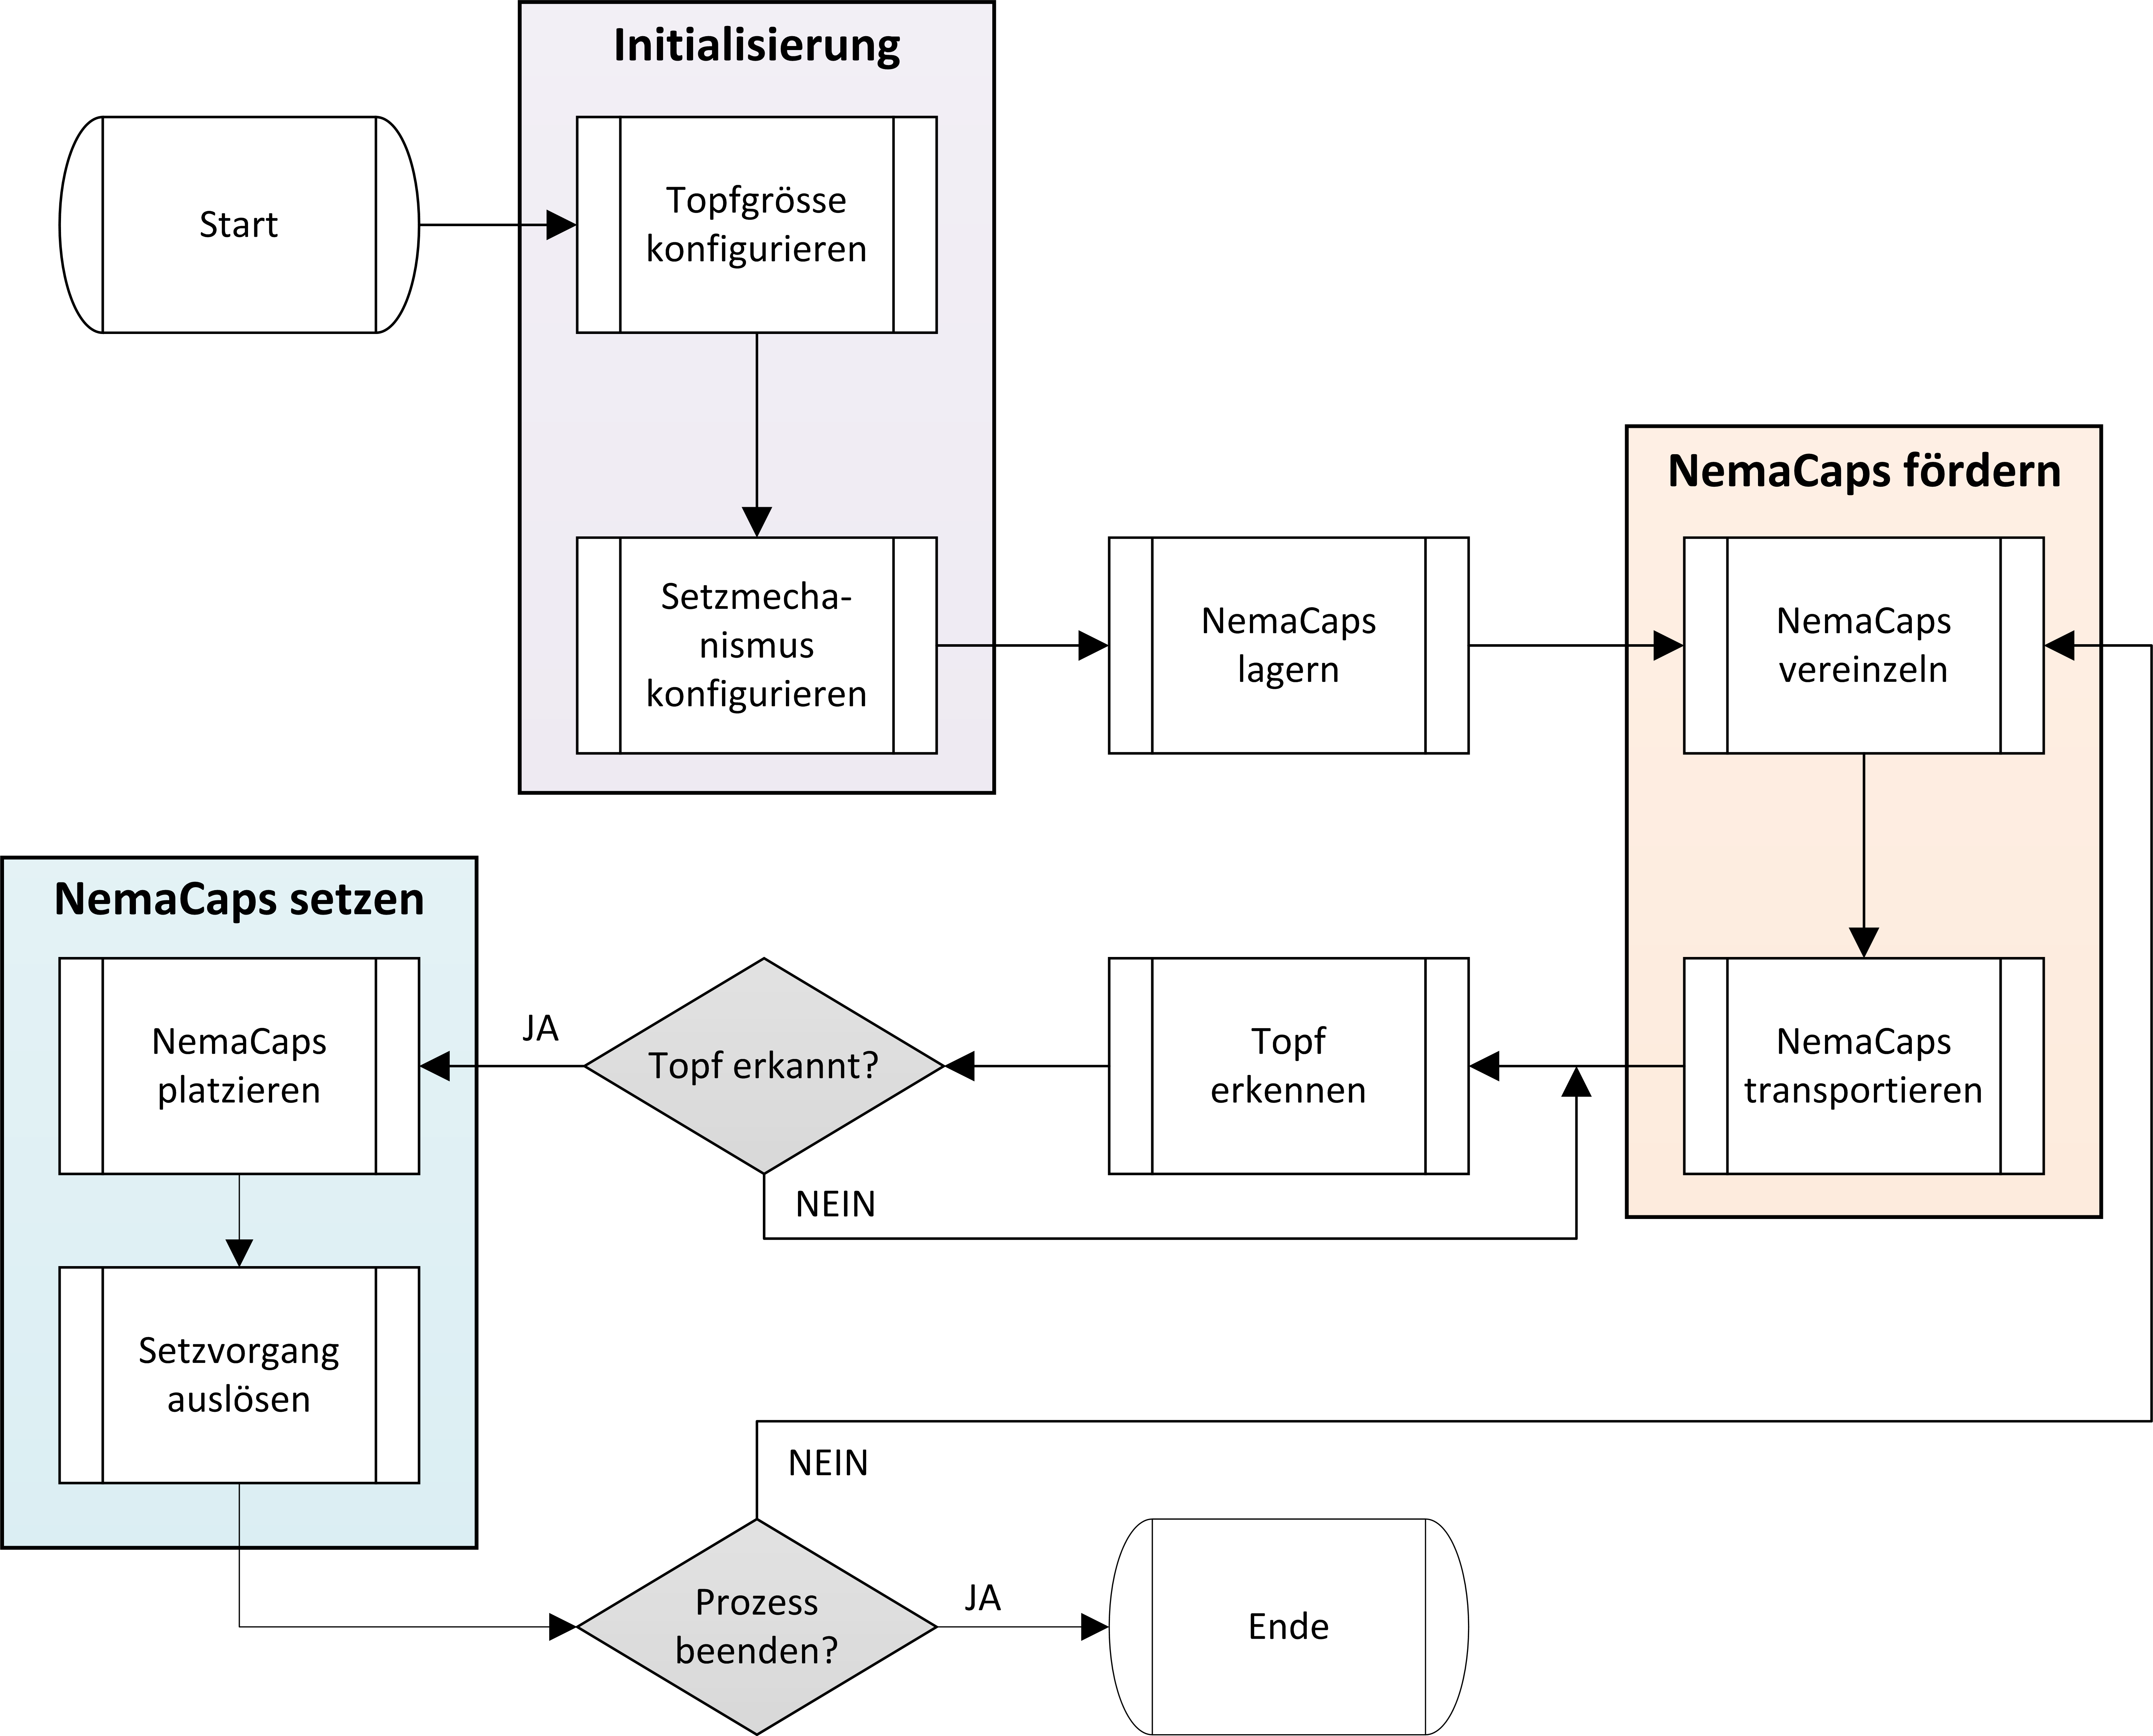
\includegraphics[width=1\textwidth]{Illustrationen/2-Funktionsanalyse/Funktionsanalyse_Pflicht.png}
	\caption{Funktionsanalyse Pflicht Blockdiagramm}
	\label{fig:FunktPflicht}
\end{figure}

\begin{itemize}
	\item \textbf{Initialisierung:} Die Initialisierung wird von einem Operator ausgeführt. Dieser Block ist nur in der Pflichtanforderung vorhanden, da die Maschine im Umfang der Pflichtanforderung die Initialisierung nicht selbstständig durchführt.
	
	\begin{itemize}
		\item \textbf{Topfgrösse konfigurieren:} In diesem Funktionsblock wird an der Maschine über ein HMI die verwendete Topfgrösse eingestellt.

		\item \textbf{Setzmechanismus konfigurieren:} Der Setzmechanismus muss für verschiedene Topfgrössen eingestellt oder ausgetauscht werden.
	\end{itemize}
	
	\item \textbf{NemaCaps lagern:} Das Setzgut (NemaCaps) wird in der Maschine mit einem Bestand von bis zu 10'000 Einheiten gelagert.
	
	\begin{figure}[H]
		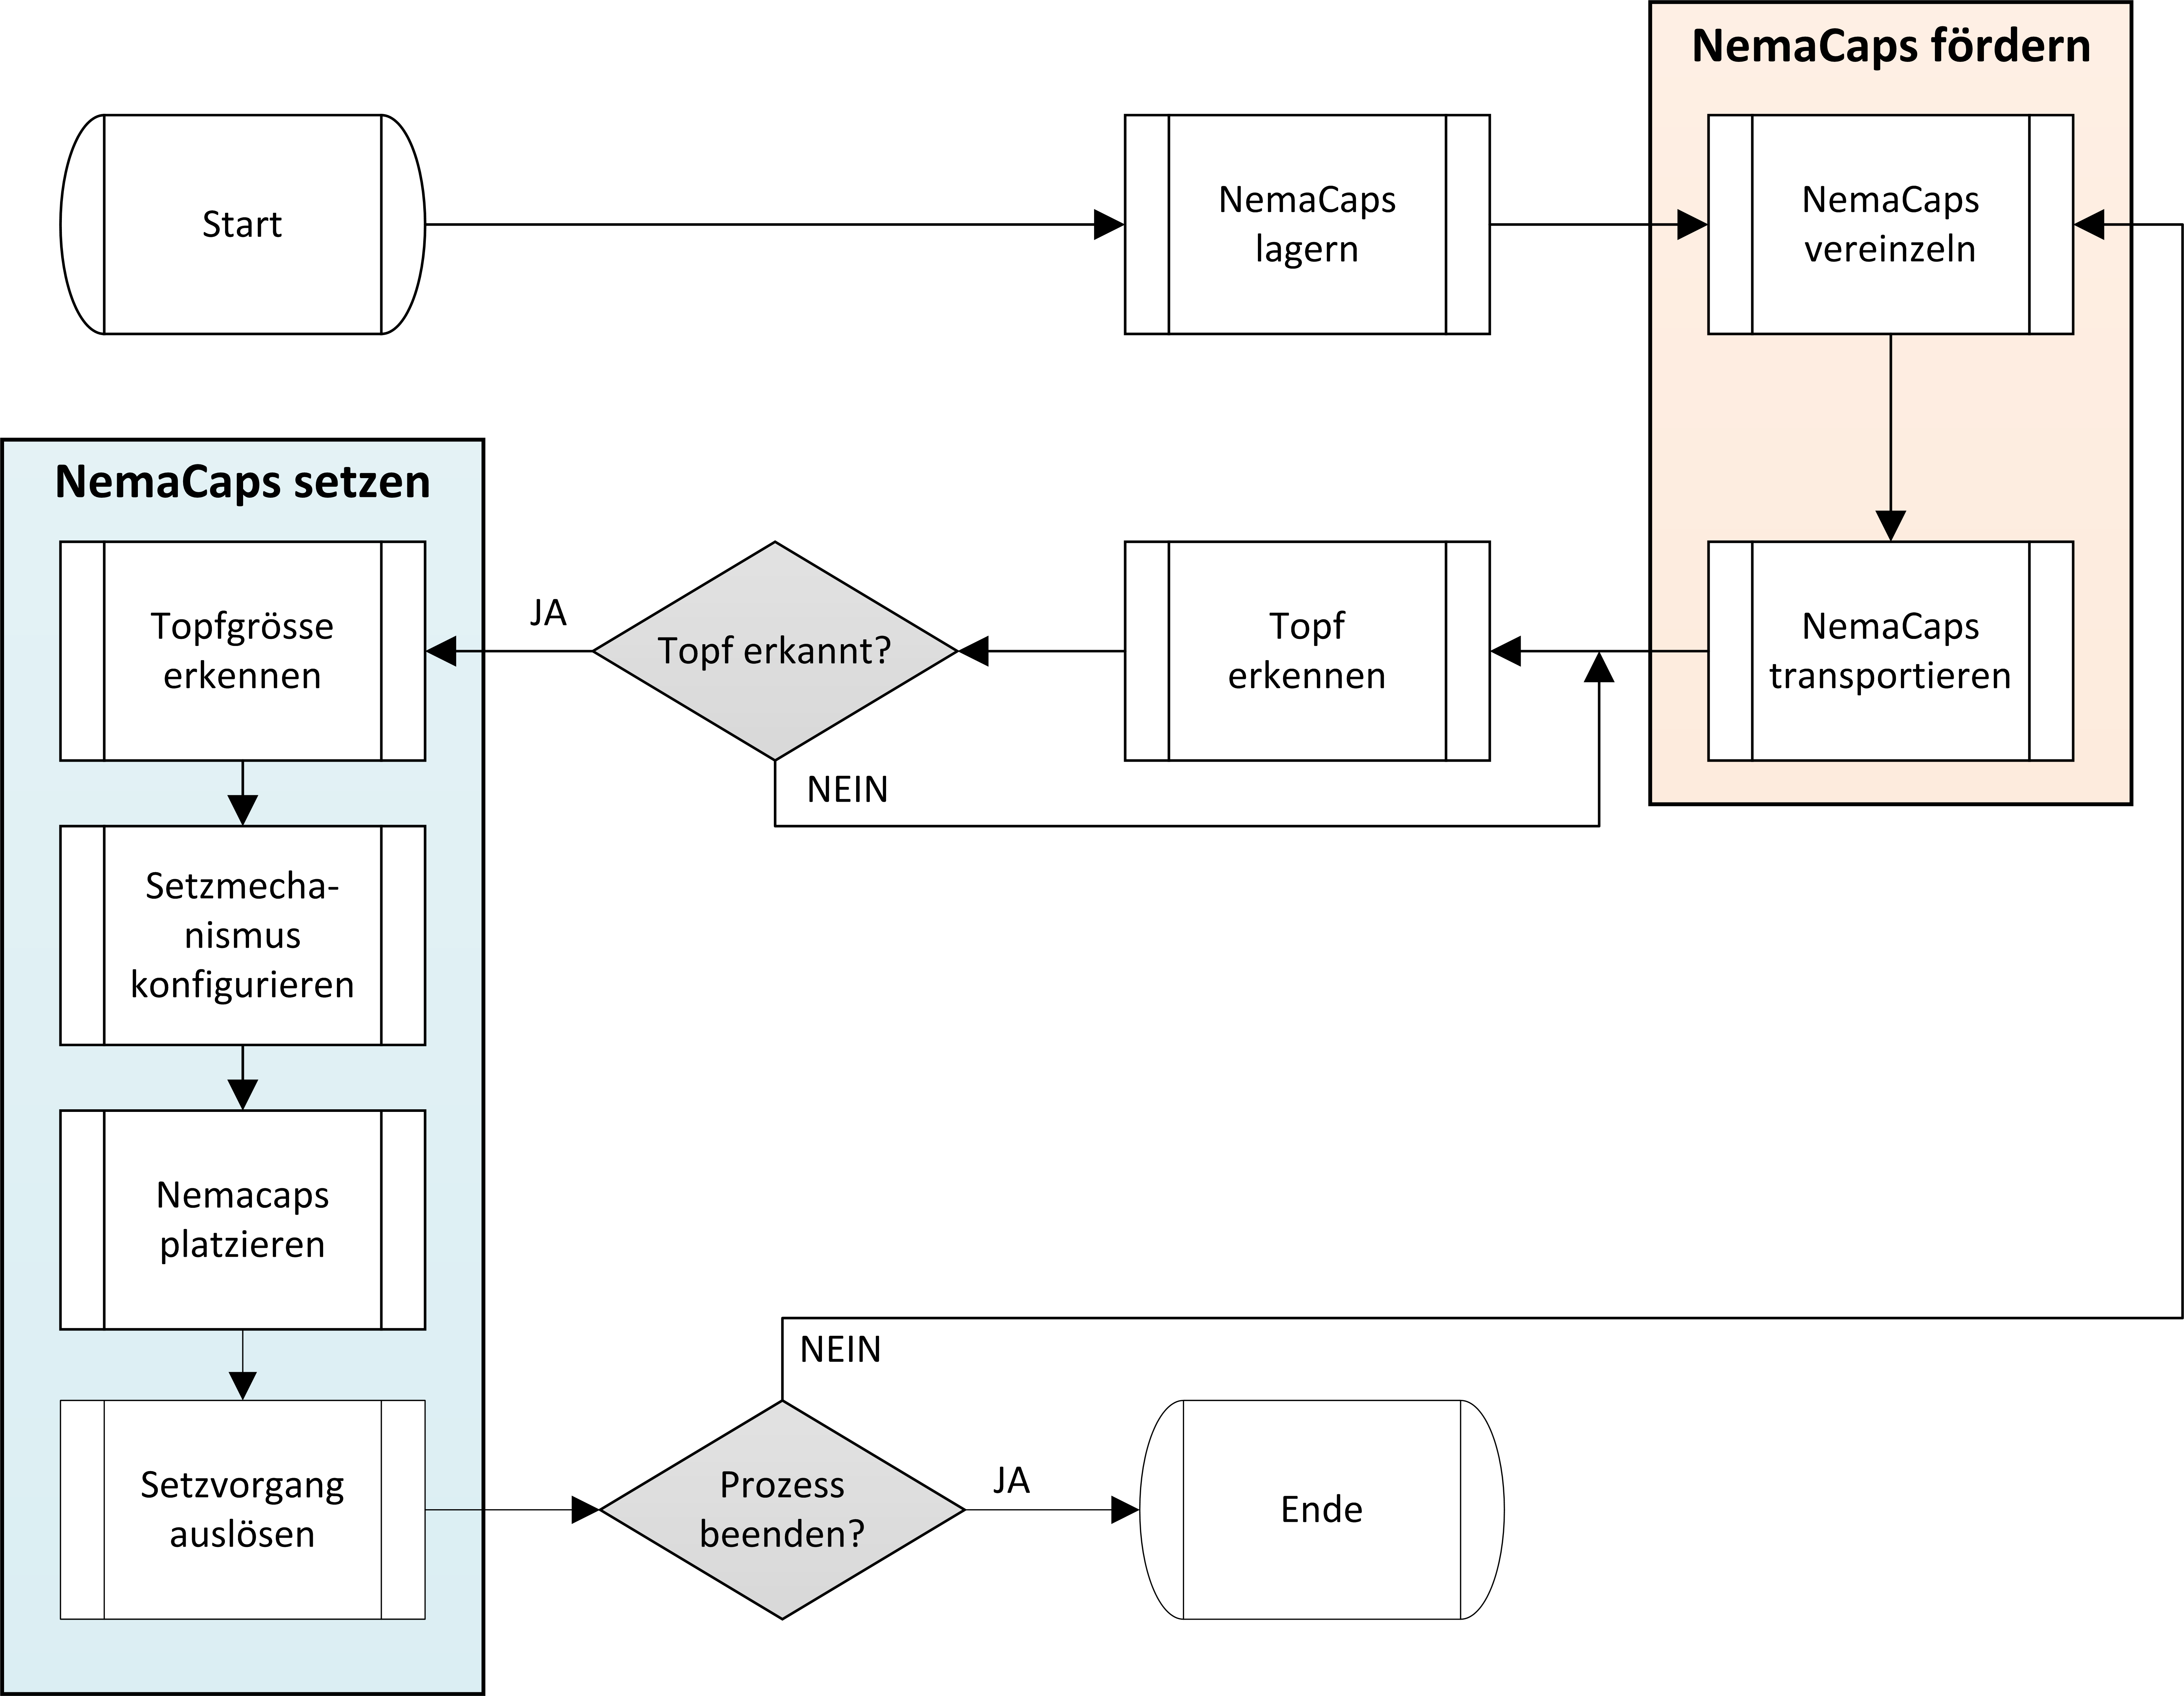
\includegraphics[width=1\textwidth]{Illustrationen/2-Funktionsanalyse/Funktionsanalyse_Wunsch.png}
		\caption{Funktionsanalyse Wunsch Blockdiagramm}
		\label{fig:FunktWunsch}
	\end{figure}
	
	\item \textbf{NemaCaps fördern:} Dieser Block behandelt die Verbindung zwischen Lager und Setzmechanismus.
	
	\begin{itemize}
		\item \textbf{NemaCaps vereinzeln:} Um die NemaCaps gezielt und kontrolliert in die Topferde einsetzen zu können, sollen diese vor dem Setzen vereinzelt werden.
		
		\item \textbf{NemaCaps transportieren:} Der Transport zwischen Lager und Setzmechanismus kann vor oder nach der Vereinzelung stattfinden.
	\end{itemize}




	\item \textbf{Topf erkennen:} Dieser Block übernimmt implizit zwei Aufgaben. Es soll erkannt werden ob überhaupt ein Topf für den Setzprozess bereit steht und ob sich dieser bewegt oder still steht. 
	
	\item \textbf{NemaCaps setzen:} Erst wenn ein Topf bereit steht wird der Setzprozess eingeleitet. Dieser unterscheidet sich wie in Abb. \ref{fig:FunktPflicht} und Abb. \ref{fig:FunktWunsch} ersichtlich zwischen Pflicht und Wunschanforderung anhand des Funktionsumfangs.
	
	\begin{itemize}
		\item \textbf{Topfgrösse erkennen:} Durch Sensorik soll die Topfgrösse jedes Topfes vermessen werden.
		
		\item \textbf{Setzmechanismus konfigurieren:} Anhand der gewonnen Daten zur Topfgrösse, soll die Maschine den Setzmechanismus selbstständig adaptieren.
		
		\item \textbf{Nemacaps platzieren:} Es folgt der eigentliche Setzprozess, in welchem die Nemacaps in einer definierten Anordnung in Position gebracht werden.
		
		\item \textbf{Setzvorgang auslösen:} Die Nemacaps welche vorher in Position gebracht wurden, werden nun in diesem Schritt vom Setzmechanismus in die Erde befördert.
	\end{itemize}
	
\end{itemize}


\newpage
\section{Einleitung}
Hexiwear ist eine von Mikroelektronika entwickelte Sensor Platform mit OLED-Display, umfangreichen Softwarefunktionen und vielen weiteren Komponenten. Die Hard- sowie Software rund um die Hexiwear wird im Umfang dieses Projektes erweitert, damit sie als universeller Sensor- und Aktorknoten für zukünftige Projekte verwendet werden kann. Weiter wird zu Demonstrationszwecken eine Hausautomations Steuerung mit der Software openHAB auf einem Raspberry Pi eingerichtet und mit der Hexiwear verknüpft. Abb. \ref{fig:komp_abstrakt} bietet eine Übersicht über die verwendeten Komponenten und deren Beschaltung.

\begin{figure}[H]
	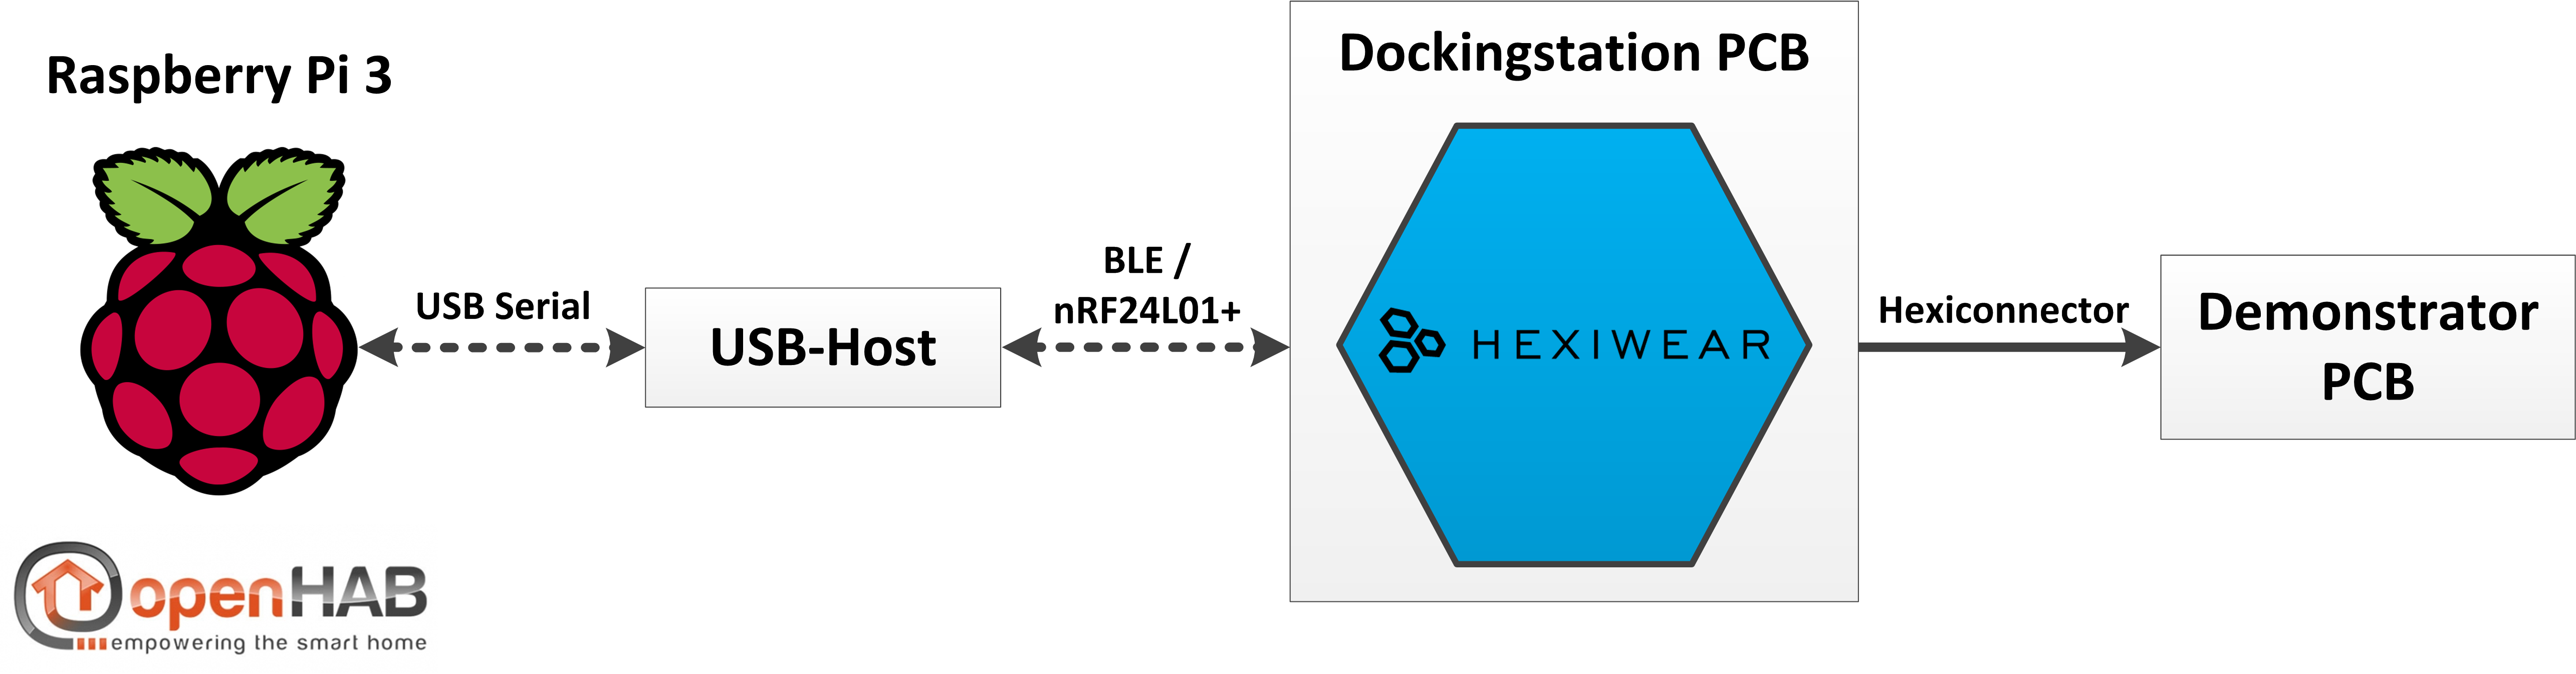
\includegraphics[width=1\textwidth]{Illustrationen/1-Einleitung/Komponentenuebersicht_grob.png}
	\caption{abstrahiertes Blockschaltbild}
	\label{fig:komp_abstrakt}
\end{figure}

Der Projektablauf kann grob in vier Teile mit entsprechenden Arbeitspaketen gegliedert werden. In Abb. \ref{fig:projektplan} ist der Projektplan in Form eines Ablaufdiagramms gemäss den vier Teilen: Initialphase, PCB, Hexiwear und Raspberry Pi / openHAB dargestellt. Der detaillierte Projektplan kann im Anhang nachgeschlagen werden.

\begin{figure}[H]
	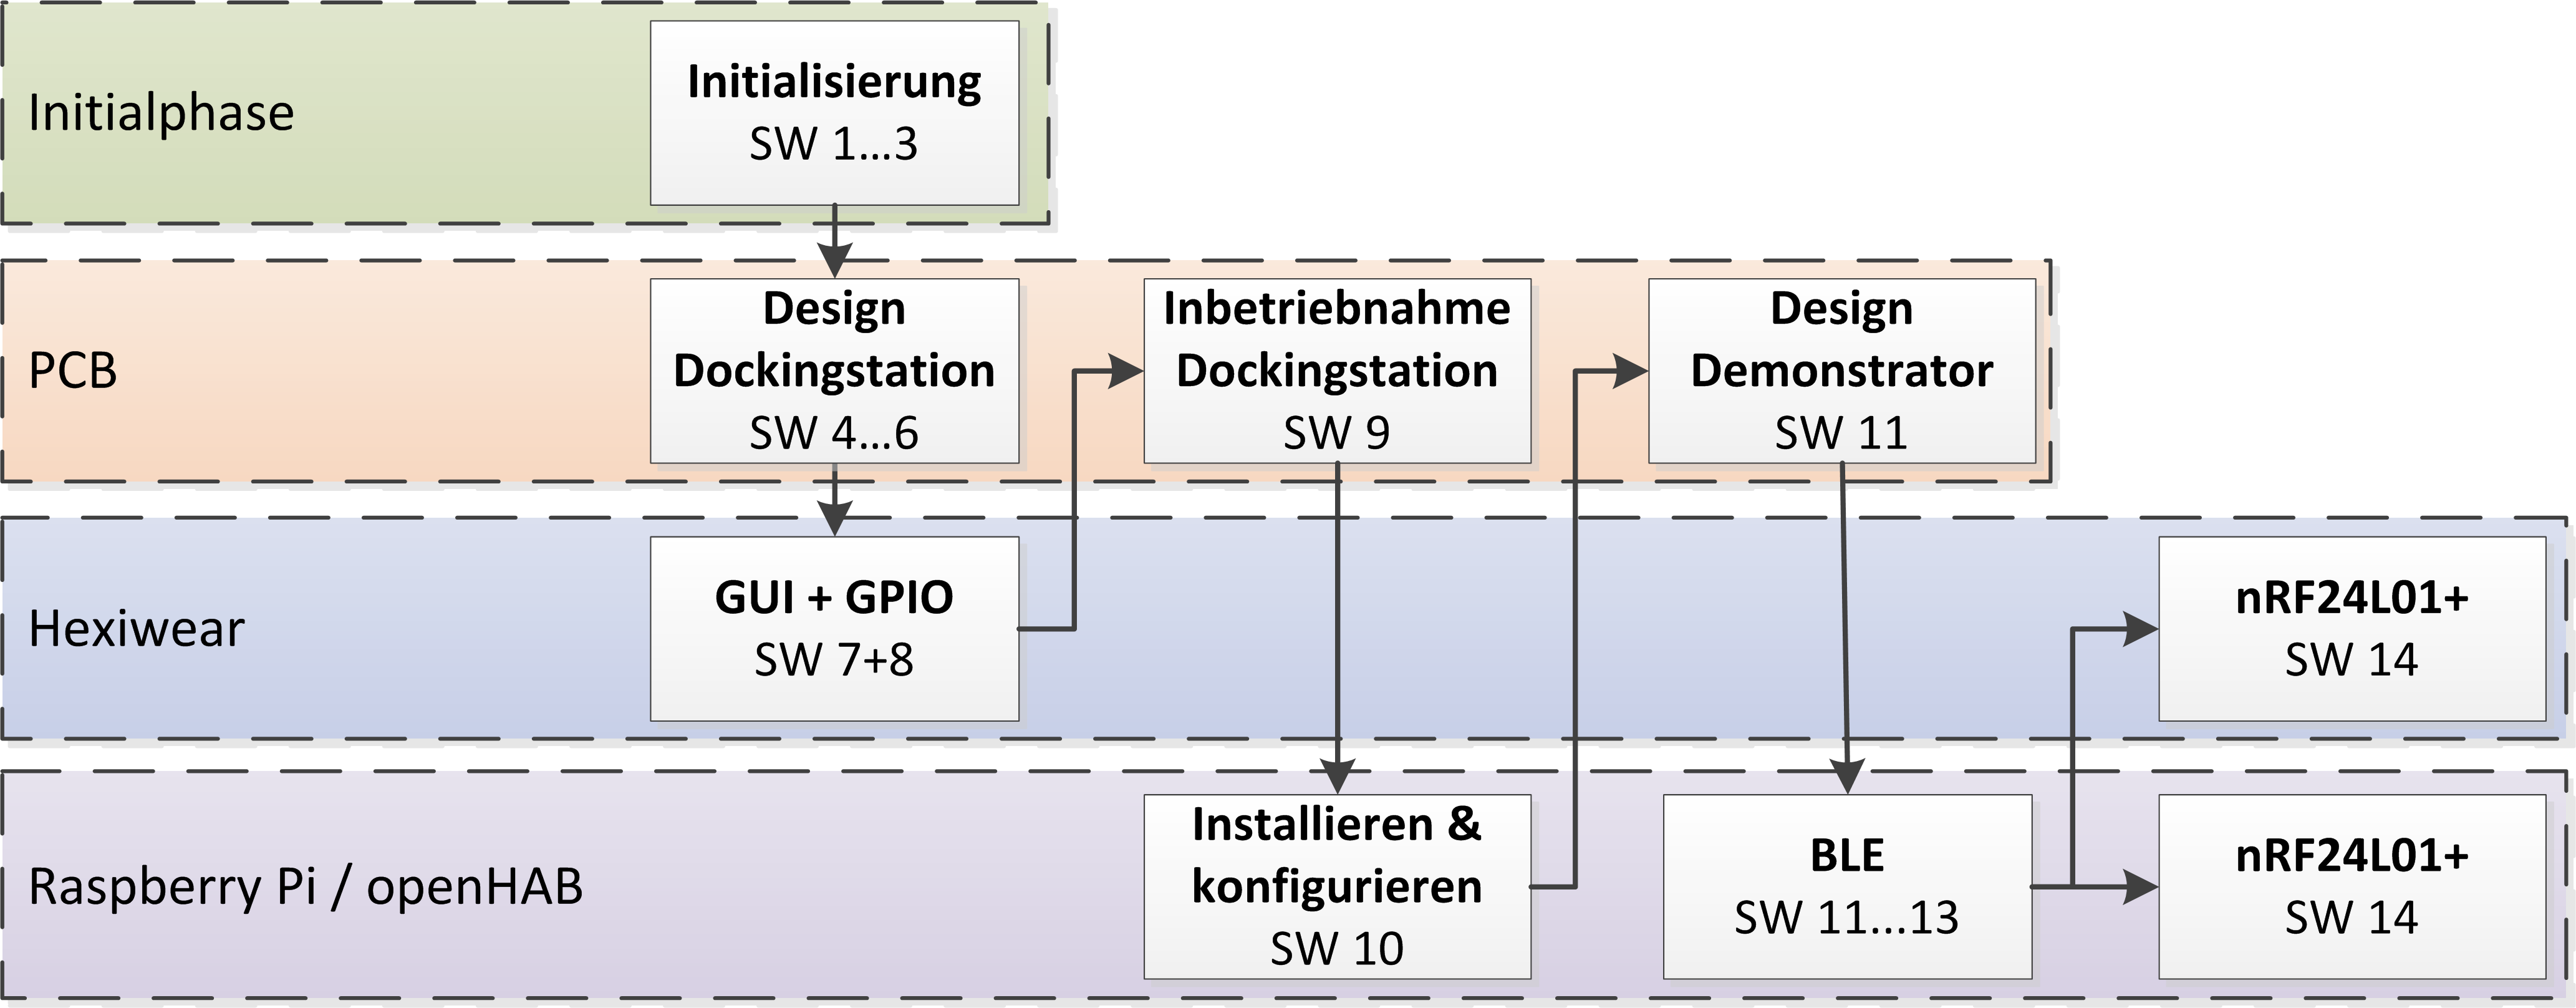
\includegraphics[width=1\textwidth]{Illustrationen/1-Einleitung/Zeitplan.png}
	\caption{Projektplan Ablaufdiagramm}
	\label{fig:projektplan}
\end{figure}

Die verschiedenen Arbeitspakete werden im folgenden Abschnitt kurz erläutert:
\begin{itemize}
	\item \textbf{Initialisierung:} Der Anfang des Projekts gestaltete sich durch einlesen in die Aufgabenstellung sowie einer Technologierecherche über die zu verwendende Hard- und Software. Weiter wurden die Dokumente zur Projektplanung und Dokumentation aufgesetzt. Da die Projektdokumentation in Latex verfasst wurde, war ein entsprechendes Selbststudium nötig. Zum Schluss der Initialphase wurde das Pflichtenheft ausgearbeitet und dem Dozenten vorgelegt.
	
	\item \textbf{Design Dockingstation:} Dieses Arbeitspaket umfasst das Zeichen des Schemas, evaluieren der Komponenten sowie das Layouten der Schaltung. Nach Abschluss des Designs wurde das PCB als Prototyp zur Fertigung an der HSLU aufgegeben. Die durch den Fertigungsprozess entstandene Wartezeit wurde mit dem nächsten Arbeitspaket überbrückt.
	
	\item \textbf{GUI + GPIO:} Zur Halbzeit des Semesters wurde die Software der Hexiwear erweitert. Dabei wurde ein neuer GUI Screen designt und eingebunden. Dieser wurde mit zwei Funktionbuttons zur Ansteuerung von LEDs versehen.
	
	\item \textbf{Inbetriebnahme Dockinstation:} Das PCB wurde bestückt und in Betrieb genommen. Sämtliche Funktionen des PCBs wurden dabei getestet.
	
	\item \textbf{Installation \& Konfiguration:} Die Software openHAB wurde auf dem Raspberry installiert und konfiguriert. Dabei wurde bereits eine Sitemap eingerichtet mit der die Hexiwear später verknüpft werden soll.
	
	\item \textbf{Design Demonstrator:} Um die Funktion der Smart-Home Applikation präsentieren zu können wurde die Schaltung für ein Demonstrator PCB designt, das Layout erstellt und das PCB zur Fertigung in Auftrag gegeben. Nach der Fertigung konnte das PCB bestückt und getestet werden.
	
	\item \textbf{BLE:} Das Arbeitspaket BLE stellte sich als sehr Zeitintensiv heraus. Zum Thema musste viel recherchiert und ausprobiert werden. Desshalb wurde das Arbeitspaket nach drei Wochen abgebrochen und eine Ist-Aufnahme durchgeführt.
	
	\item \textbf{nRF24L01+:} Zum Schluss wurde der alternative drahtlos Kommunikationspfad nRF24L01+ mit tatkräftiger Unterstützung des Dozenten auf der Hexiwear und dem Raspberry Pi implementiert. Dabei wurde auf dem Raspberry das Mikrocontrollerboard USB-Host über USB angeschlossen. Dieses Arbeitspaket konnte ebenfalls Mangels Zeit nicht Fertiggestellt werden.
\end{itemize}
\newpage
\section{Schlussdiskussion und Persönliches Fazit}
\subsection{Schlussdiskussion}



\subsection{Persönliches Fazit}




\newpage

\bibliography{Quellen/literatur}
\newpage
\begin{appendix}
\section{Anhang}
Folgende Dokumente befinden sich in schriftlicher Form im Anhang:

\begin{itemize}
	\item \verb|Aufgabenstellung|
\end{itemize}

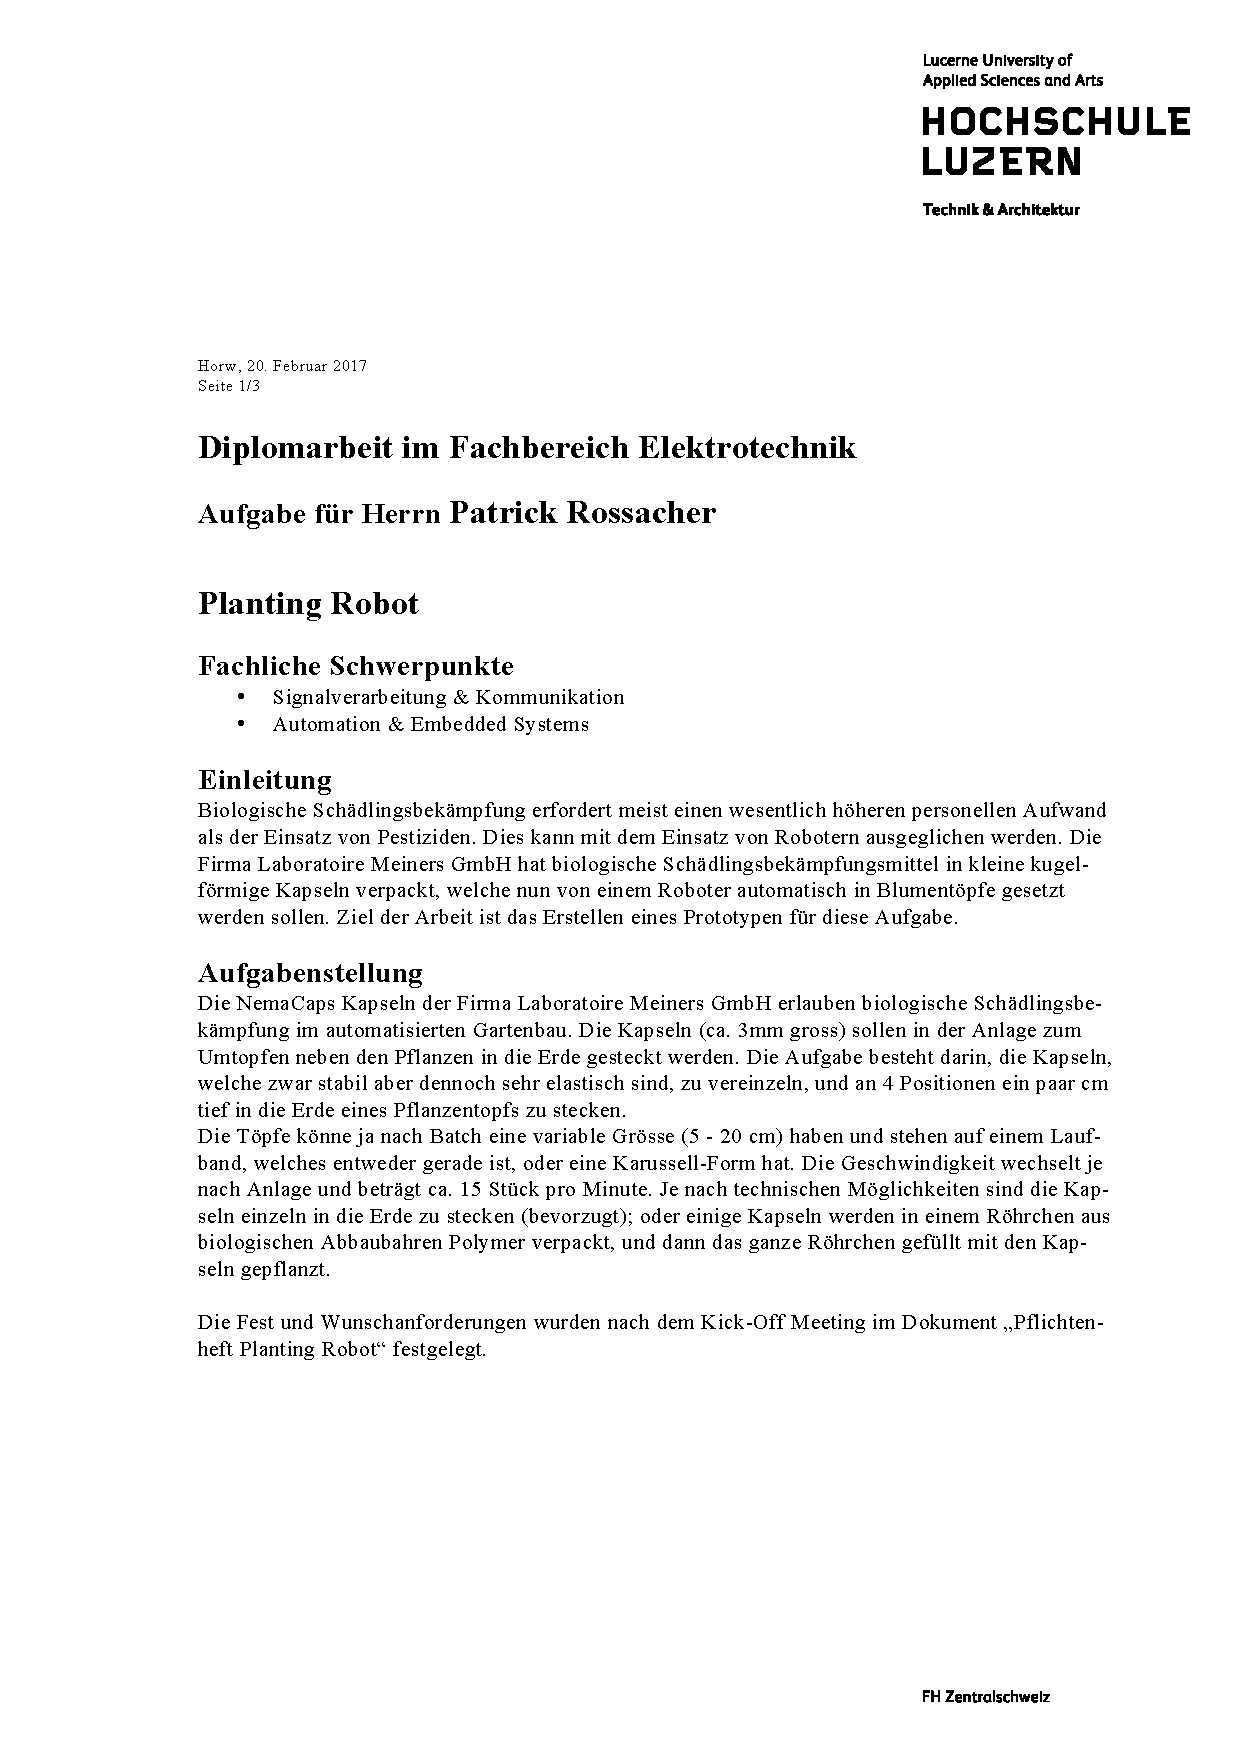
\includepdf[pages=-,nup=1x1]{Illustrationen/6-Anhang/Aufgabenstellung.pdf}


\end{appendix}
\end{document}